\documentclass[beamer]{standalone}
\usepackage{../templates/common}
\usetikzlibrary{patterns}

\begin{document}
\begin{standaloneframe}
\centering
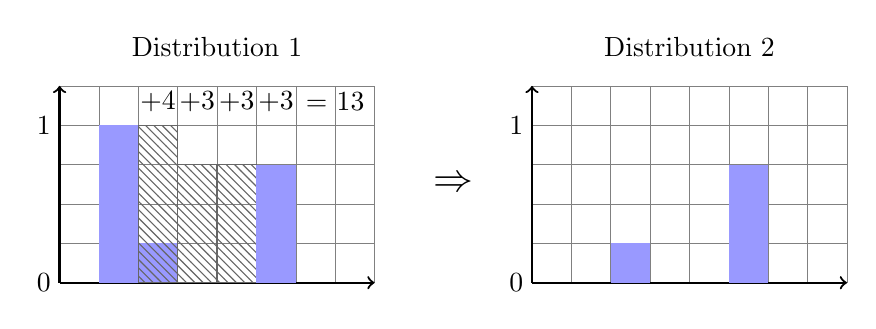
\begin{tikzpicture}
\node at (2,3) {Distribution 1};
\node at (8,3) {Distribution 2};
\node at (5,1.25) {\Large $\Rightarrow$};
\draw (-.2,2) node  {1};
\draw (-.2,0) node  {0};
\draw[step=0.5cm,gray,very thin] (-0,-0) grid (4,2.5);
\draw[thick, ->] (0,0) -- (0,2.5);
\draw[thick, ->] (0,0) -- (4,0);

\fill<1>[blue!40!white] (.5,0) rectangle (1,2);%

\fill<3->[blue!40!white] (1,0) rectangle (1.5,.5);
\draw<2>[pattern=north west lines, pattern color=black!60, draw=black!60] (1,0) rectangle (1.5,2);%2
\draw<2-> (1.25,2.3) node  {+4};


\draw<3>[pattern=north west lines, pattern color=black!60, draw=black!60] (1.5,0) rectangle (2,1.5);%3
\draw<3-> (1.75,2.3) node  {+3};

\draw<4>[pattern=north west lines, pattern color=black!60, draw=black!60] (2,0) rectangle (2.5,1.5);%4
\draw<4-> (2.25,2.3) node  {+3};


\fill<5>[blue!40!white] (2.5,0) rectangle (3,1.5);
\draw<5> (2.75,2.3) node  {+3};
\draw<5> (3.5,2.3) node  {= 13};

\draw (6-.2,2) node  {1};
\draw (6-.2,0) node  {0};
\draw[step=0.5cm,gray,very thin] (6,-0) grid (10,2.5);
\draw[thick, ->] (6,0) -- (6,2.5);
\draw[thick, ->] (6,0) -- (10,0);
\fill[blue!40!white] (7,0) rectangle (7.5,.5);
\fill[blue!40!white] (8.5,0) rectangle (9,1.5);
\end{tikzpicture}
\end{standaloneframe}
\end{document}
